\begin{frame}
\frametitle{Statistics}
The general process of investigation has 4 stages:
\begin{enumerate}
\item Identify a question or problem.
\item Collect relevant data on the topic.
\item Analyze the data.
\item Form a conclusion.
\end{enumerate}
We hope to make stages 2-4 objective, rigorous, and efficient.

How best can we collect data? How
should it be analyzed? And what can we infer from the analysis?
\end{frame}



\begin{frame}
\frametitle{Our intuitions are often wrong}
``Common sense is nothing more than a deposit of prejudices laid down by the mind before you reach age 18.'' - Albert Einstein

\pause

``Common sense is what tells us the earth is flat.'' - Stuart Chase

\pause

\vspace{20pt}

\dq{Together, a bat and ball cost $\$1.10$. The bat costs $\$1.00$ {\bf more} than the ball. How much does the ball cost?}

\soln{\pause{The ball costs 5 cents.}}
\end{frame}

\begin{frame}
\frametitle{Incorrect intuitions - survivorship bias}
In WWII, the Center for Naval Analyses considered adding armor to planes.

\pause 
 
\begin{itemize}
\item When planes returned after getting hit by bullets, the locations were documented.

\pause
\item The figure below characterizes the locations of bullet holes in the planes that returned.
\begin{center}
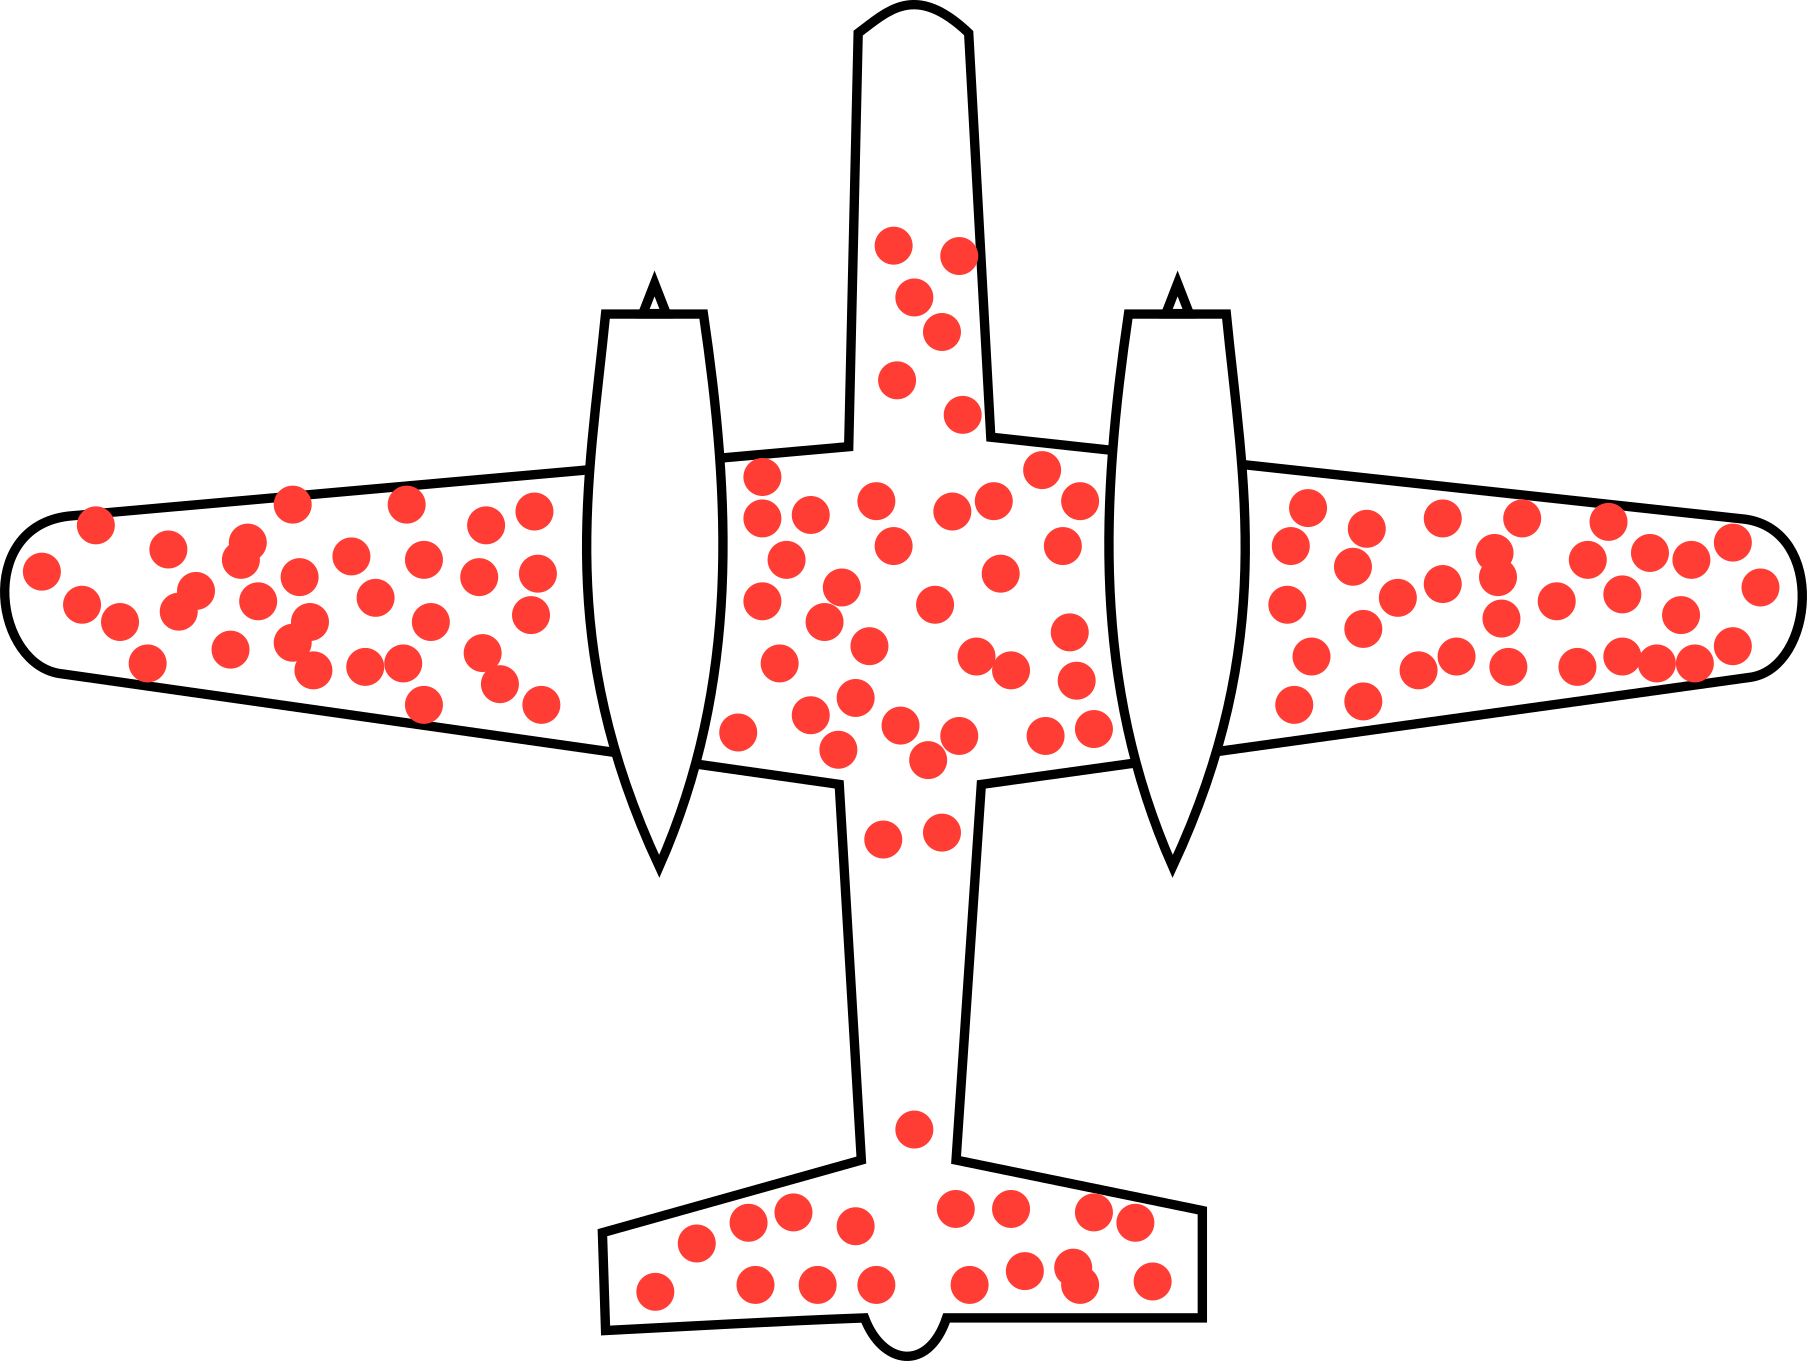
\includegraphics[scale=0.25]{1-1_case_study/figures/plane}
\end{center}
\end{itemize}

\dq{Where should armor be added?}
\soln{\pause{Add armor where holes are {\bf not} located (engines, cockpit, and tail).}}
\end{frame}


\begin{frame}
\frametitle{This class will {\bf not} be intuitive.}
\begin{itemize}
\item This class will {\bf not} be intuitive.
\pause
\item You will need to practice.
\pause
\item A lot.
\end{itemize}
\end{frame}





%%%%%%%%%%%%%%%%%%%%%%%%%%%%%%%%%%%%

\section{Case study}

%%%%%%%%%%%%%%%%%%%%%%%%%%%%%%%%%%%%


\begin{frame}
\frametitle{Using Stents to Prevent Strokes}

\begin{itemize}
\item Objective: Evaluate the effectiveness of stents in preventing strokes.

\item Treatment group: Patients in the treatment group received a stent and medical management. The medical management included medications, management of risk factors, and help in lifestyle modification.
\item Control group: Patients in the control group received the same medical management as the treatment group, but they did not receive stents.
\end{itemize}

\ct{Chimowitz MI, Lynn MJ, Derdeyn CP, et al. 2011. Stenting versus Aggressive Medical Therapy for Intracranial Arterial Stenosis. New England Journal of Medicine 365:993-1003.}
\end{frame}

\begin{frame}
\frametitle{Results of Using Stents to Prevent Strokes}
\begin{table}[h]
\centering
\begin{tabular}{l c cc}
	&& 	stroke 	& no event \\
  \hline
treatment 	&&	45 	& 179 \\
control 		&& 	28	& 199 \\
  \hline
Total		&&	73	& 378 \\
  \hline
\end{tabular}
\caption{Descriptive statistics for the stent study (after 1 year).}
\label{stentStudyResults}
\end{table}

\pause
\dq{What proportion of treatment group had a stroke?}
\soln{\pause{$\frac{45}{45+179} =$  20\%}}

\pause
\dq{What proportion of control group had a stroke?}
\soln{\pause{$\frac{28}{28+199} =$ 12\%}}

\end{frame}

\begin{frame}
\frametitle{Understanding the results}

\dq{Do the data show a ``real'' difference between the groups?}

\pause

\begin{itemize}

\item Suppose you flip a coin 100 times. While the chance a coin lands heads in any given coin flip is 50\%, we probably won't observe exactly 50 heads. This type of fluctuation is part of almost any type of data generating process.

\item The observed difference between the two groups (20 - 12 = 8\%) may be real, or may be due to natural variation.

\item We need statistical tools to determine if the difference is so large that we should reject the notion that it was due to chance.

\end{itemize}

\end{frame}




\begin{frame}
\frametitle{Treating Chronic Fatigue Syndrome}

\begin{itemize}

\item Objective: Evaluate the effectiveness of cognitive-behavior therapy for chronic fatigue syndrome.

\item Participant pool: 142 patients who were recruited from referrals by primary care physicians and consultants to a hospital clinic specializing in chronic fatigue syndrome.

\item Actual participants: Only 60 of the 142 referred patients entered the study. Some were excluded because they didn't meet the diagnostic criteria, some had other health issues, and some refused to be a part of the study.

\end{itemize}

\ct{Deale et. al. \textit{Cognitive behavior therapy for chronic fatigue syndrome: A randomized controlled trial}. The American Journal of Psychiatry 154.3 (1997).}

\end{frame}

%%%%%%%%%%%%%%%%%%%%%%%%%%%%%%%%%%%%

\begin{frame}
\frametitle{Study design}

\begin{itemize}

\item Patients randomly assigned to treatment and control groups, 30 patients in each group:
\begin{itemize}
\item \hl{Treatment}: Cognitive behavior therapy -- collaborative, educative, and with a behavioral emphasis. Patients were shown on how activity could be increased steadily and safely without exacerbating symptoms.
\item \hl{Control:} Relaxation -- No advice was given about how activity could be increased. Instead progressive muscle relaxation, visualization, and rapid relaxation skills were taught.
\end{itemize}

\end{itemize}

\end{frame}

%%%%%%%%%%%%%%%%%%%%%%%%%%%%%%%%%%%%

\begin{frame}
\frametitle{Results}

The table below shows the distribution of patients with good outcomes at 6-month follow-up. Note that 7 patients dropped out of the study: 3 from the treatment and 4 from the control group.

\begin{center}
\begin{tabular}{ll  cc c} 
			&				& \multicolumn{2}{c}{\textit{Good outcome}} \\
\cline{3-4}
			&							& Yes 	& No 	& Total	\\
\cline{2-5}
							&Treatment 	& 19	 	& 8		& 27 	\\
\raisebox{1.5ex}[0pt]{\textit{Group}}	&Control		& 5	 	& 21	 	& 26 \\
\cline{2-5}
							&Total		& 24		& 29		& 53
\end{tabular}
\end{center}

\pause

\begin{itemize}

\item Proportion with good outcomes in treatment group:
\[ 19 / 27 \approx 0.70 \rightarrow 70\% \]

\pause

\item Proportion with good outcomes in control group:
\[ 5 / 26 \approx 0.19 \rightarrow 19\% \]

\end{itemize}

\end{frame}

%%%%%%%%%%%%%%%%%%%%%%%%%%%%%%%%%%%%

\begin{frame}
\frametitle{Understanding the results}

\dq{Do the data show a ``real" difference between the groups?}

\pause

\begin{itemize}

\item Suppose you flip a coin 100 times. While the chance a coin lands heads in any given coin flip is 50\%, we probably won't observe exactly 50 heads. This type of fluctuation is part of almost any type of data generating process.

\item The observed difference between the two groups (70 - 19 = 51\%) may be real, or may be due to natural variation.

\item Since the difference is quite large, it is more believable that the difference is real.

\item We need statistical tools to determine if the difference is so large that we should reject the notion that it was due to chance.

\end{itemize}

\end{frame}

%%%%%%%%%%%%%%%%%%%%%%%%%%%%%%%%%%%%

\begin{frame}
\frametitle{Generalizing the results}

\dq{Are the results of this study generalizable to all patients with chronic fatigue syndrome?}

\pause

These patients had specific characteristics and volunteered to be a part of this study, therefore they may not be representative of all patients with chronic fatigue syndrome. While we cannot immediately generalize the results to all patients, this first study is encouraging. The method works for patients with some narrow set of characteristics, and that gives hope that it will work, at least to some degree, with other patients.


\end{frame}

%%%%%%%%%%%%%%%%%%%%%%%%%%%%%%%%%%%%
